\documentclass[11pt]{article}
\usepackage{graphicx} % This lets you include figures
\usepackage{hyperref} % This lets you make links to web locations
\usepackage[margin=0.5in]{geometry}
\usepackage[rightcaption]{sidecap}
\usepackage{subcaption}
\usepackage{wrapfig}
\usepackage{float}
\usepackage{imakeidx}
\usepackage{indentfirst}
\makeindex
\usepackage{listings}
\lstset{
  basicstyle=\ttfamily\footnotesize,
  breaklines=true,
  breakatwhitespace=false,
  numbers=left,
  numberstyle=\tiny,
  stepnumber=1,
  numbersep=5pt
}
%---------------------------Do Not Edit Anything Above This Line!!------------------------

% edit the line below, if needed, to change the directory name for your image files.
\graphicspath{ {./images/} }
\setlength{\parindent}{0pt}


\begin{document}

%---------------------------Edit Content in the Box to Create the Title Page--------------
\begin{titlepage}
   \begin{center}
       \vspace*{1cm}
	   \Huge
       \textbf{Automated Testing Framework for a Distributed Disaster Response System }

       \vspace{0.5cm}
       \Large
       Project 2 \\
       9-30-2025 \\
   \end{center}

       \vspace{1.5cm}

\begin{table}[h!]
\centering
\begin{tabular}{|l|l|}
\hline
\textbf{Name} & \textbf{Email Address} \\ \hline
Nate Barner& nathaniel.barner603@topper.wku.edu\\ \hline
Kaden Hunt& kaden.hunt144@topper.wku.edu\\ \hline
\end{tabular}
\end{table}

%Latex Table Generator    
%https://www.tablesgenerator.com/     
        
\vspace{4in}

\centering        
CS 396 \\
Fall 2025\\
Project Technical Documentation

\end{titlepage}
%---------------------------Edit Content in the Box to Create the Title Page--------------


% No text here.


%---------------------------Do Not Edit Anything In This Box!!------------------------
%Table of contents and list of figures will be autogenerated by this section.
\newpage
\setcounter{page}{1}%
\cleardoublepage
\pagenumbering{gobble}
\tableofcontents
\cleardoublepage
\pagenumbering{arabic}
\clearpage
\newpage
\setcounter{page}{1}%
\cleardoublepage
\pagenumbering{gobble}
\listoffigures
\cleardoublepage
\pagenumbering{arabic}
\newpage
%---------------------------Do Not Edit Anything In This Box!!------------------------




%---------------------------Project Introduction Section------------------------------

% No text here.

\section{Introduction} %\section{} is used to create major section headers

% No text here.

%---------------------------Project Overview------------------------------------------
\subsection{Project Overview} %\subsection{} is used to create minor sections 
% 300 words
% Description of the project, what the project provides, its purpose, problems solved, and target audience.

This project is a test automation framework designed to improve the quality of code in applications. Our project will use a disaster response system as the application to test. The framework provides a structured way to design, execute, and report on unit and integration tests. The framework's primary purpose is to catch errors or defects in the code quickly, speed up the development workflow and give confidence to developers making software changes.\\
%use blank lines to begin a new paragraph

The framework has three key capabilities. First, it provides automated unit testing to find any errors for individual functions ensuring that small components behave as expected. Second, it enables integration testing that validates separate modules together, confirming data and control flow across system. Third it includes system testing to imitate real user scenarios, showing that the application works correctly from end to end.\\

Along with test execution, the framework allows for quick management of test cases, developers can create, edit, and run tests at all times. directly integrated with GitHub actions to create a CI/CD pipeline; allowing for automatic testing for every code commit and pull request. This process will then generate detailed reports for all tests. Test reports will contain data on coverage, pass/fail results, and data trends. These generated reports are saved as artifacts and will be further parsed into one comprehensive testing results report.\\

This framework solves common software development problems such as manual testing which is time consuming and difficult to scale. By making testing automatic and making them part of the development cycle we reduce human error, increase consistency and feedback while providing developers with confidence of system reliability.\\

The audience for this framework is developer teams making distributed systems, where reliability is very important. Another audience is for students learning software development practices with a emphasis on DevOps and the advantages of continuous integration and development.\\
%---------------------------End Project Overview---------------------------------------

% No text here.

%---------------------------Project Scope----------------------------------------------
\subsection{Project Scope}
% 350 words
% Description of all deliverables, benefits, outcomes, and work required (all tasks, costs, time, people, resources, dates/deadlines, and final deliverables date).

The scope of this project is to design and implement a lightweight DevOps test automation framework for a distributed disaster response coordination system. The framework will demonstrate unit, integration, and system testing through Python and pytest, integrated into a GitHub Actions CI/CD pipeline. The project emphasizes early defect detection, code quality assurance, and efficient feedback for developers.\\

\textbf{Deliverables.}  
The final submission will include: (1) a GitHub repository containing the source code, test framework, and configuration files; (2) automated test suites for unit, integration, and system-level testing; (3) a GitHub Actions pipeline that installs dependencies, executes the test suites, generates coverage metrics, and uploads test artifacts; (4) documentation consisting of technical and organizational reports, a README, and test strategy notes; (5) presentation slides; and (6) a recorded demonstration video. The project folder will be compressed and submitted through Blackboard.\\

\textbf{Benefits and Outcomes.}  
This project provides a robust, reusable automation workflow that reduces manual testing effort and improves software reliability. Outcomes include consistent code validation on every commit, improvements in test coverage, and practical experience with DevOps practices. Teams benefit from faster feedback loops, reduced deployment risks, and an organized approach to software quality.\\

\textbf{Work Required.}  
Tasks involve setting up the repository and environment, designing test cases for core components, building integration tests for cross-module interactions, configuring the CI pipeline, generating coverage and results reports, preparing documentation, and creating the demo presentation. The work also requires drafting technical and organizational documents in LaTeX, assembling slides, and recording the video demo. All work will be completed collaboratively by the two team members, with shared responsibility for development, testing, and documentation.\\

\textbf{People and Resources.}  
The project team consists of Kaden Hunt and Nate Barner. No external costs are expected. Required resources include GitHub (for repository hosting and Actions), Python 3.11, pytest, and coverage tools. Documentation will be prepared with LaTeX.\\

\textbf{Schedule.}  
The assignment was given on September 9, 2025, and all deliverables are due on September 30, 2025. The Gantt chart will illustrate milestones such as environment setup, pipeline implementation, testing, documentation, and demo preparation. The final deliverables will be complete and submitted by the deadline.\\

%---------------------------End Project Scope---------------------------------------

% No text here.


\subsection{Technical Requirements}


%---------------------------Functional Requirements----------------------------------------------
\subsubsection{Functional Requirements} %\subsubsection{} used to create sections for parent subsections.
% Functional requirements define what a system or software must do, specifying the desired behavior or functionality.

% List as atomic bullet points that can be tested

\begin{table}[H]
\centering
\begin{tabular}{|l|}
\hline
\textbf{Mandatory Functional Requirements} \\ \hline
Support automated unit testing of 
disaster\_app components in isolation.      \\ \hline
Provide automated integration testing that validates data flow across modules                                       \\ \hline
Execute automated system-level testing covering end-to-end emergency handling                                      \\ \hline
Offer structured test-case management for creating, updating, and organizing scenarios                                           \\ 
                                        \hline
Integrate with CI/CD to trigger test runs on each push or pull request                                           \\ \hline
\textbf{Extended Functional Requirements}  \\ \hline
Generate combined results, coverage, and historical trends for quality tracking                                \\ \hline
Ship a CLI runner to list or execute cases by ID or type for targeted validation                                 \\ \hline
Archive artifacts and auto-commit refreshed reports during main-branch builds                                 \\ \hline
\end{tabular}
\end{table}

% Paragraph (150 words) explaining the need and purpose for the listed Functional Requirements.
The functional requirements define what actions the  framework must fulfill. Unit tests provide a way to check each disaster\_app function by itself, catching mistakes right when they happen. Integration tests show that modules can communicate with each other without data getting lost or corrupted, and system tests walk through entire scenarios end-to-end. To keep cases organized, we used JSON files and a simple CLI runner so new tests can be added without touching the harness itself. Finally, tying all of this into GitHub Actions means every commit runs the suite automatically and produces a new final report, so we can see right away if something broke. Together, these requirements make sure testing is a constant part of the workflow.\\


%---------------------------End Functional Requirements----------------------------------------------

% No text here.

%---------------------------Non-Functional Requirements----------------------------------------------
\subsubsection{Non-Functional Requirements}
% Non-functional requirements specify the constraints, qualities, or attributes that the system or software must possess, such as performance, security, usability, portability, fault tolerance, or reliability.

% List as atomic bullet points that can be tested

\begin{table}[H]
\centering
\begin{tabular}{|l|}
\hline
\textbf{Mandatory Non-Functional Requirements} \\ \hline
Implement logging and error handling across core logic and reporting pipeline                                      \\ \hline
Complete automated regression suite within less than 5 minutes performance target                                      \\ \hline
Scale via JSON-defined scenarios and CLI filters\\ \hline
Protect sensitive artifacts by excluding reports and environment-specific files from version control                                           \\ \hline
Provide an on-boarding experience with documentation and tooling.                                           \\ \hline
\textbf{Extended Non-Functional Requirements}  \\ \hline
Maintain historical test trend data for proactive monitoring                                 \\ \hline
Publish coverage and JUnit artifacts automatically for team transparency                                 \\ \hline

\end{tabular}
\end{table}

% Paragraph (150 words) explaining the need and purpose for the listed Non-Functional Requirements.
The non-functional requirements cover how the framework behaves rather than what it does. All logging and error handling are built into both the disaster\_app logic and in the reporting pipeline so failures are clear and fixable. The test suite is lightweight, nine quick tests that finish well under the five-minute window in CI. Because scenarios are defined in JSON and can be filtered by the runner, the framework scales by simply dropping in new files. Security features protect sensitive outputs like reports and environment files by leaving them out of version control but they are still available as build artifacts for review. Clear setup instructions and readable CLI output make the framework approachable for new developers and reliable for repeat use.\\



%---------------------------End Non-Functional Requirements---------------------------------------

% No text here.



%---------------------------DevOps - Continuous Delivery Approach and Results-------------------------------------------------

\section{DevOps - Continuous Integration and Continuous Delivery Approach and Results}
%describe your set of practices that enable you to release software quickly, safely, and sustainably by automating the software delivery process, resulting in faster time to market, improved software quality, and enhanced team productivity.
Every push or pull request to main triggers the CI workflow automatically. Dependencies install, pytest runs with coverage, and make\_report.py combines results into a single report. Artifacts like JUnit XML, coverage data, and history logs are uploaded. On main-branch pushes, updated reports are committed back so history always lines up with the codebase. This setup gives us quick feedback and keeps test results from getting out of sync.
 tx\\


%---------------------------End DevOps - Continuous Delivery Approach and Results-------------------------------------------------



%---------------------------DevOps - Architecture Approach, Models, and Results-------------------------------------------------

\section{DevOps - Architecture Approach, Models, and Results}
%describe how you designed systems with loosely coupled components, allowing you to work independently, deploy frequently, and scale efficiently, ultimately enabling rapid delivery of software and system reliability.
The project uses a modular design. Core functions handle parsing, assigning responders, updating, and sending alerts, with a simple lock in place to prevent conflicts. Each of these pieces can be tested on its own through unit tests. Integration and system tests then show how those parts fit together, from a single emergency to a queue of multiple ones. The separation makes it easy to expand the framework without everything breaking at once.

%---------------------------End DevOps - Architecture Approach, Models, and Results-------------------------------------------------



% No text here.

%---------------------------DevOps - Product and Process Approach and Results-------------------------------------------------

\section{DevOps - Product and Process Approach and Results}
%describe your focus on creating customer-centric, feedback-driven development processes that integrate cross-functional teams, enabling continuous improvement and alignment between product development and business outcomes.
Our process focused on being repeatable and transparent. Requirements were mapped directly to tests so it’s easy to trace what’s being verified. The runner, JSON catalog, and CI steps give us a consistent path: when a new test case is added, it follows the same process from local run to automated build. That consistency reduces mistakes and makes reviews more straightforward. The runner, JSON catalog, and CI steps enforce a repeatable delivery process where each case promotion follows the same tooling path, reducing manual error.



%---------------------------End DevOps - Product and Process Approach and Results-------------------------------------------------

% No text here.


%---------------------------DevOps - Product Management and Monitoring Approach and Results-------------------------------------------------

\section{DevOps - Product Management and Monitoring Approach and Results}
%describe how you implemented proactive, data-driven monitoring and feedback systems that provide real-time insights into system performance, enabling you to identify issues early, improve decision-making, and optimize both system stability and team performance.
We didn’t want test results to disappear after each run, so make\_report.py saves them to history.json and prints out a short trend summary. Over time this shows whether coverage is slipping or pass rates are dropping. That level of monitoring gives us a check on quality and helps guide what to improve next.

%---------------------------End DevOps - Product Management and Monitoring Approach and Results-------------------------------------------------


% No text here.

%---------------------------Product DevOps - Cultural Approach and Results-------------------------------------------------

\section{DevOps - Cultural Approach and Results}
%describe how your team created a collaborative, trust-based environment that emphasizes shared responsibility, continuous learning, and experimentation, driving high performance and innovation.
The project team, made up of Kaden Hunt and Nate Barner, divided tasks according to strengths while keeping responsibilities balanced. Kaden focused on CI/CD setup, dependency management, and reporting automation, while Nate concentrated on the disaster response application and test case design. Both worked together on documentation and deliverables.

Decisions were made collaboratively, and failures were treated as shared issues rather than individual mistakes. This encouraged experimentation, steady progress, and a culture of trust. By combining teamwork habits with DevOps automation, feedback was visible to both contributors and ownership of results was shared. This approach kept accountability high and reinforced continuous learning throughout the project.






%---------------------------End DevOps - Cultural Approach and Results-------------------------------------------------


% No text here.

%---------------------------Software Product Testing Section-------------------------------------
\section{Software Testing and Results}

\subsection{Testing}

The software testing process validated the disaster response application through unit, integration, and system tests. Using Pytest, we ensured that each function, such as parsing reports, assigning responders, and sending alerts, worked correctly both individually and together in workflows. Automated testing through GitHub Actions provided continuous integration, ensuring tests ran consistently across environments. A coverage report confirmed 100\% code coverage, demonstrating that all logic paths were exercised. Screenshots of test results, coverage analysis, and workflow outputs document this process. Overall, testing verified the system’s correctness, robustness, and reliability under simulated real-world scenarios.

\subsection{Results}

Figure 1 shows the results of running our full test suite. Each test function executed successfully, covering unit, integration, and system tests. The output confirms that no failures occurred, demonstrating that the application performs as expected across multiple scenarios and edge cases.

\begin{figure} [H]
    \centering
    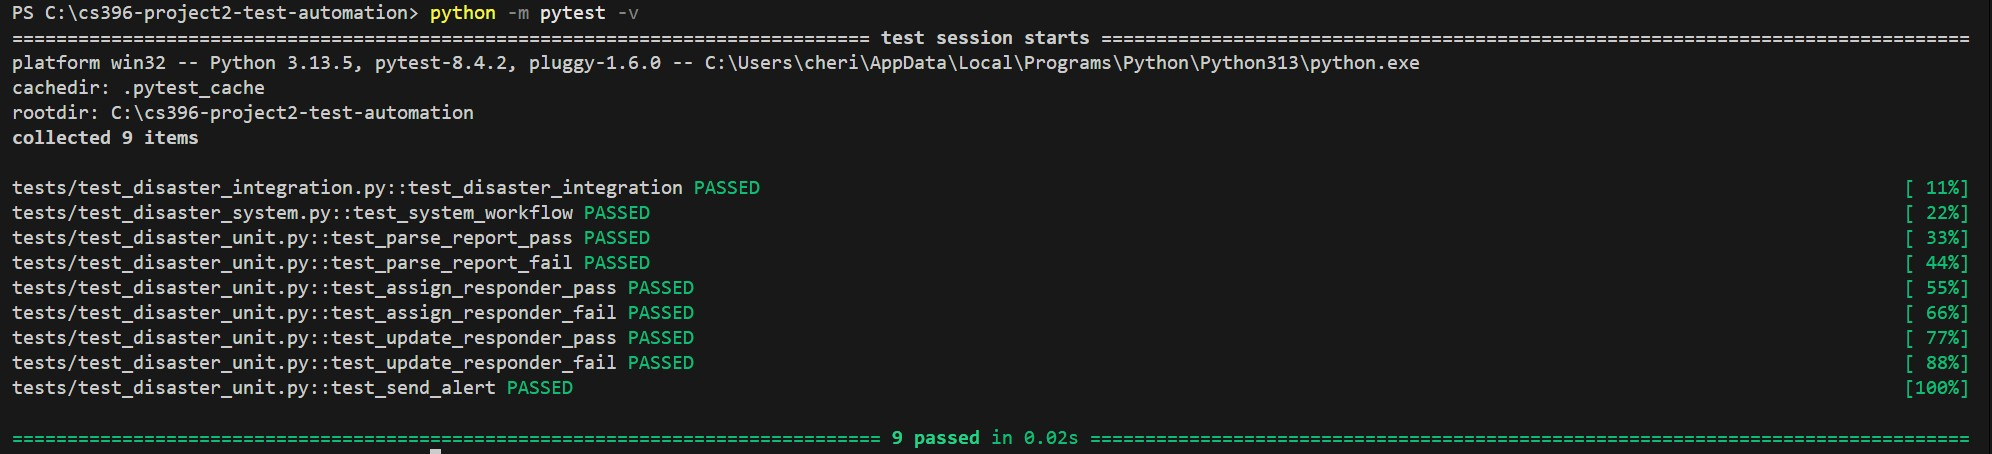
\includegraphics[width=0.75\linewidth]{images/test_results.jpg}
    \caption{Pytest Output}
    \label{fig:test_results}
\end{figure}

This screenshot, Figure 2, provides the test coverage report for the project. The results confirm 100\% coverage, meaning every line of code in disaster\_app.py was executed during testing. This demonstrates thorough validation of the core logic and strengthens confidence in the project’s reliability and correctness.

\begin{figure}[H]
    \centering
    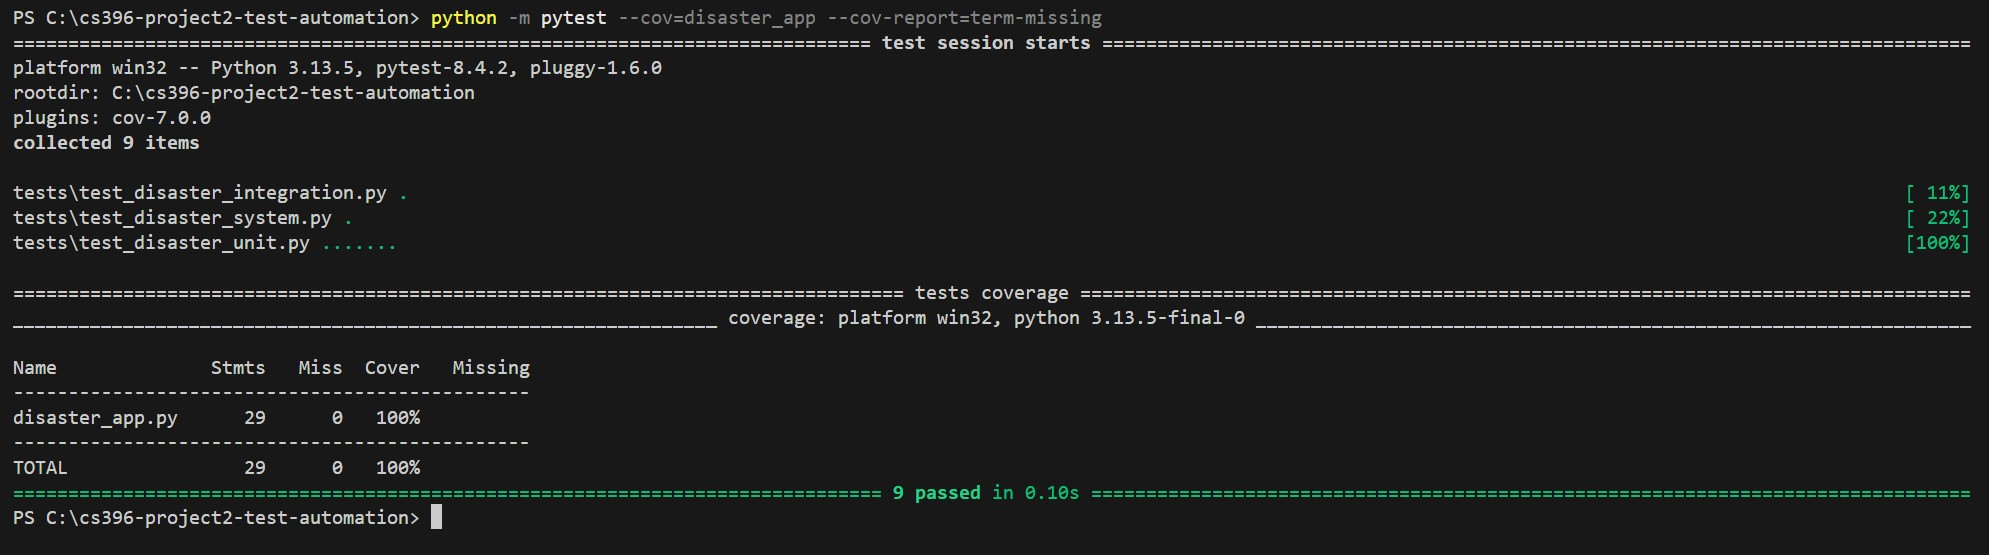
\includegraphics[width=0.75\linewidth]{images/test_coverage.jpg}
    \caption{Coverage report in the terminal}
    \label{fig:coverage}
\end{figure}

The screenshot below, Figure 3, captures the automated testing pipeline running through GitHub Actions. The successful status confirms that all code passed testing in a continuous integration environment. This ensures tests are consistent across environments, validates automation setup, and provides confidence in code quality.

\begin{figure}[H]
    \centering
    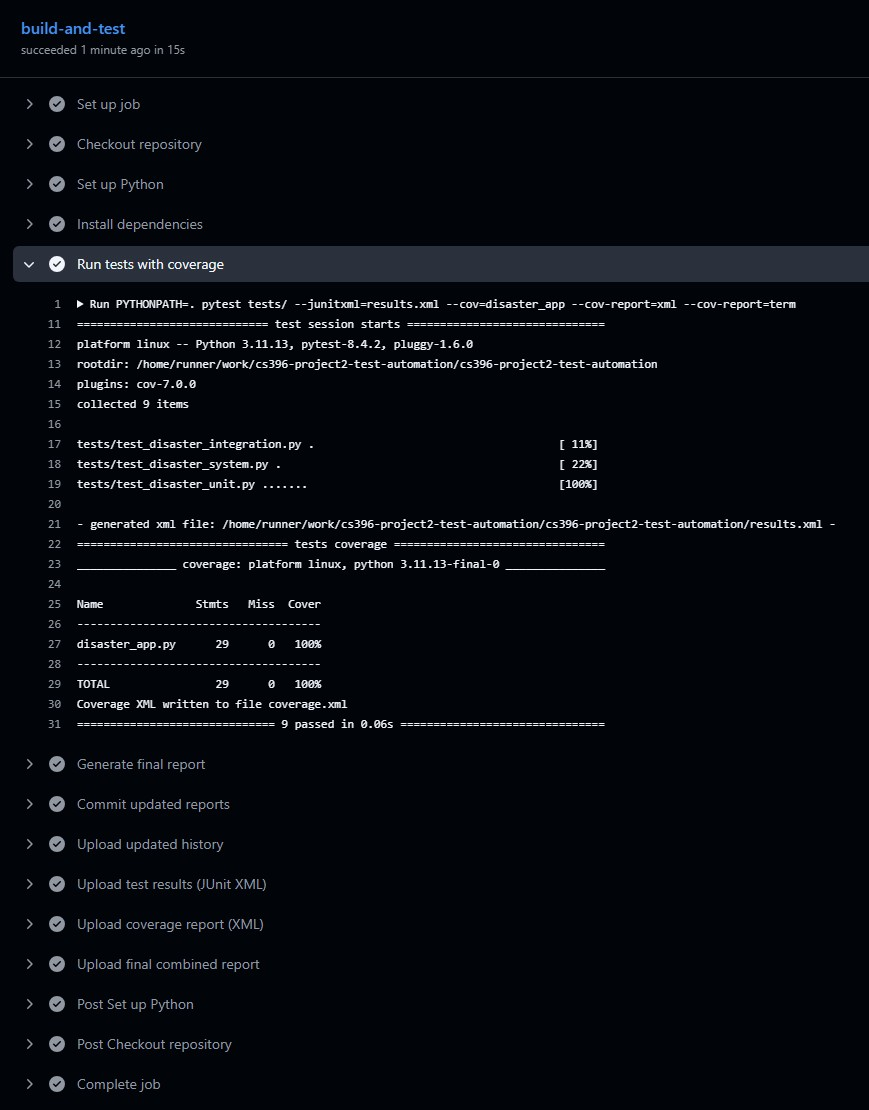
\includegraphics[width=0.5\linewidth]{images/workflow.jpg}
    \caption{GitHub Actions workflow run}
    \label{fig:placeholder}
\end{figure}

The framework generates a machine-readable JSON report that records test execution results and coverage details. Below is Figure 4, the raw JSON file:

\begin{figure} [H]
    \centering
    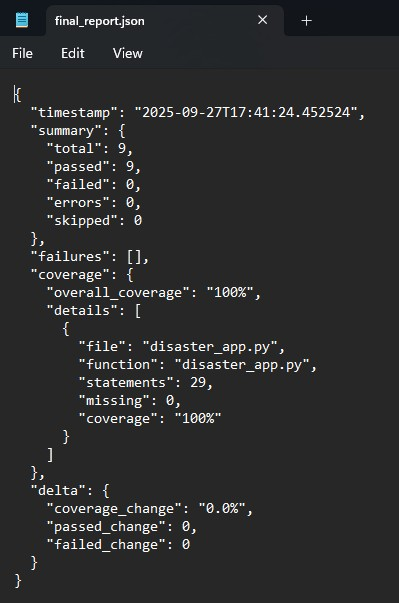
\includegraphics[width=0.34\linewidth]{images/final_report_json.jpg}
    \caption{Final Report JSON}
    \label{fig:placeholder}
\end{figure}

To make the results clearer, the data is summarized in the following table:

\begin{table}[h!]
\centering
\begin{tabular}{|l|c|}
\hline
\textbf{Metric} & \textbf{Value} \\
\hline
Total Tests      & 9      \\
Passed           & 9      \\
Failed           & 0      \\
Errors           & 0      \\
Skipped          & 0      \\
Overall Coverage & 100\%  \\
\hline
\end{tabular}
\caption{Summary of automated test results and code coverage.}
\end{table}

This shows that all nine tests passed successfully with no errors or failures, and the application code is fully covered by the test suite.
%---------------------------Software Testing Plan Template-------------------------------------

\subsection{Software Testing Plan Template}
%Each of the testing levels (unit, Integration, System, Acceptance) should use the following test plan template.

\textbf{Test Plan Identifier:} %Provides a unique identifier for the test. Every test should have a unique identification number for reference.
T001: Unit Testing

\textbf{Introduction:} % 50 words. Brief description and objective about the test type.
Unit testing ensures that each individual function in the disaster response application works correctly by itself. This testing focuses on input parsing, responder assignment, status updates, and alert generation independently, detecting defects early and confirming that each small part of the system behaves as expected before combining them into workflows.

\textbf{Test item:} %50 words. Includes detailed information about the Software Under Test (SUT).
The software under test includes four main functions: parse\_emergency\_report, assign\_responder, update\_responder, and send\_alert. Each function is tested independently to verify correct input handling, expected outputs, and proper error handling. This testing excludes interactions with external services or multi-function workflows, focusing purely on isolated function behavior.

\textbf{Features to test/not to test:} %50 words. In scope features. This could be newly added or updated features. Out of scope features not tested. [Provide reasoning for exclusion, like, non-impacted, low priority, etc.]
Tested features: parsing emergency reports, assigning responders, updating responder status, and sending alerts. Out-of-scope features: system-level workflows, multiple simultaneous emergencies, and network communication. These are excluded because unit testing targets individual functions, allowing fast feedback and early detection of code errors without involving larger system interactions.

\textbf{Approach:} %50 words. Strategy to test the software. Includes types of tests and how to test. Functional, performance, security testing using combined [manual + automation], manual only, automation only approach.
Automated pytest scripts test each function using valid and invalid inputs. Assertions verify outputs and exceptions are handled correctly. Only automated testing is used to provide fast, repeatable feedback. Unit tests integrate into the CI/CD pipeline to ensure that every commit triggers immediate verification of function correctness.

\textbf{Test deliverables:} %50 words. All the deliverables from the testing e.g. approaches, test cases, reports etc.
Deliverables include unit test scripts, pytest reports, coverage metrics, and logs of test execution. These artifacts demonstrate function correctness, historical trends, and areas needing improvement. They support traceability, provide evidence for grading or review, and form the foundation for higher-level testing such as integration and system tests.

\textbf{Item pass/fail criteria:} %50 words. Entry and Exit criteria for all items. 
Tests pass if all assertions succeed and expected exceptions are raised for invalid inputs. Entry criteria include code ready for testing; exit criteria require all unit tests to pass and coverage reports to be generated, demonstrating full testing of isolated function logic without failures.

\textbf{Environmental needs:} %50 words. Infrastructure required for SUT and executing test cases.
Python 3.11+, pytest, and pytest-cov installed. Tests run locally or on CI/CD (GitHub Actions) with the disaster\_app module available. No network or external dependencies are needed, keeping tests fast, isolated, and reproducible across environments.

\textbf{Responsibilities:} %50 words. Roles and responsibilities for various testing / supported activities.
Developers write and maintain unit tests. CI/CD executes tests on code changes. Team members review results, coverage, and edge cases to ensure comprehensive function verification. Leads ensure adherence to test plan and correctness of test logic.

\textbf{Staffing and training needs:} %50 words. Training needs to bridge the gap of available and expected skill.
Testers should understand Python, pytest, and unit testing principles. Training focuses on writing assertions, testing error handling, and using CI/CD for automated execution. Documentation provides guidance for consistent test development.

\textbf{Schedule:} %50 words.  Test schedule should also be noted in the Gantt Chart. Test estimation (Efforts) and high-level schedule. Schedule should be for key deliverables or important milestones. Ideally, all test deliverables included in the test plan should be scheduled.
Unit tests are executed on every commit or pull request. Initial scripts completed within the first week. Continuous expansion occurs as new functions are added. CI/CD ensures automated execution and daily review of test results for early defect detection.

\textbf{Risks and Mitigation:} %100 words. Risk identification for applicable items, assumptions, and mitigation plan.
Risks include untested edge cases and interface changes breaking tests. Mitigation involves monitoring coverage, adding additional unit tests, and reviewing tests when code changes. CI/CD provides rapid detection and resolution of failures.

\textbf{Approvals:} %Approvals and sign of dates.
Kaden Hunt – 9/12/2025
Nate Barner – 9/13/2025
\vspace{.5cm}

\textbf{Test Plan Identifier:} %Provides a unique identifier for the test. Every test should have a unique identification number for reference.
T002: Integration testing

\textbf{Introduction:} % 50 words. Brief description and objective about the test type.
Integration testing verifies that multiple components of the disaster response system work together correctly. The test ensures that parsing, responder assignment, status updates, and alerting communicate properly, with data flowing correctly between modules. Integration tests help detect interface issues, logic errors, and improper data handling early in the combined workflows.

\textbf{Test item:} %50 words. Includes detailed information about the Software Under Test (SUT).
The SUT is the combination of parse\_emergency\_report, assign\_responder, update\_responder, and send\_alert. Integration tests validate that outputs from one function are correctly received and used by the next. The focus is on interactions and data flow, excluding external services or real-time notifications for simplicity and reproducibility.

\textbf{Features to test/not to test:} %50 words. In scope features. This could be newly added or updated features. Out of scope features not tested. [Provide reasoning for exclusion, like, non-impacted, low priority, etc.]
In-scope: proper workflow of a single emergency report, correct data handoff, and status updates between modules. Out-of-scope: multiple concurrent reports, network alerts, and end-to-end system performance. These exclusions are due to the scope of integration testing, which focuses on correct communication between modules rather than full system load handling.

\textbf{Approach:} %50 words. Strategy to test the software. Includes types of tests and how to test. Functional, performance, security testing using combined [manual + automation], manual only, automation only approach.
Automated pytest scripts simulate a single emergency processed through all modules sequentially. Assertions verify that parsed data is correct, responders are assigned and updated, and alerts are generated. Automated testing ensures repeatable results and fast feedback integrated into CI/CD pipelines.

\textbf{Test deliverables:} %50 words. All the deliverables from the testing e.g. approaches, test cases, reports etc.
Integration test scripts, pytest results, JUnit XML, and coverage reports. These documents provide evidence of correct module interactions, document failed interfaces, and track trends in data handling errors or unexpected module behavior.

\textbf{Item pass/fail criteria:} %50 words. Entry and Exit criteria for all items. 
Integration passes if all modules work correctly together without exceptions, and data integrity is maintained. Entry criteria: all unit tests pass. Exit criteria: all assertions in the integration workflow pass and produce coverage reports.

\textbf{Environmental needs:} %50 words. Infrastructure required for SUT and executing test cases.
Python 3.11+, pytest, and pytest-cov installed. CI/CD environment (GitHub Actions) configured to execute integration workflows. Local testing requires disaster\_app module available. No network or external service dependencies.

\textbf{Responsibilities:} %50 words. Roles and responsibilities for various testing / supported activities.
Developers create and maintain integration scripts. CI/CD executes tests on code merges. Team reviews results, verifies data flow, and updates test scripts as modules evolve. Leads ensure workflow correctness and proper coverage of module interactions.

\textbf{Staffing and training needs:} %50 words. Training needs to bridge the gap of available and expected skill.
Testers need understanding of Python, pytest, and integration testing concepts. Training covers creating tests spanning multiple modules, handling exceptions, and analyzing module interactions.

\textbf{Schedule:} %50 words.  Test schedule should also be noted in the Gantt Chart. Test estimation (Efforts) and high-level schedule. Schedule should be for key deliverables or important milestones. Ideally, all test deliverables included in the test plan should be scheduled.
Integration tests executed on merges to main. Initial scripts completed after unit tests are verified. CI/CD ensures automation and daily review of results to catch interface errors early.

\textbf{Risks and Mitigation:} %100 words. Risk identification for applicable items, assumptions, and mitigation plan.
Interface mismatches and incorrect data flow may cause failures. Mitigation: maintain proper unit test coverage, review module contracts, and monitor integration test results. CI/CD provides rapid failure detection for early correction.

\textbf{Approvals:} %Approvals and sign of dates.
Kaden Hunt – 9/18/2025
Nate Barner – 9/18/2025
\vspace{.5cm}

\textbf{Test Plan Identifier:} %Provides a unique identifier for the test. Every test should have a unique identification number for reference.
T003: System testing

\textbf{Introduction:} % 50 words. Brief description and objective about the test type.
System testing evaluates the complete disaster response application under realistic scenarios, simulating multiple emergency reports handled simultaneously. It tests end-to-end workflows, ensuring that the system correctly assigns responders, updates their statuses, and sends alerts for all emergencies while maintaining data integrity and overall functionality.

\textbf{Test item:} %50 words. Includes detailed information about the Software Under Test (SUT).
The SUT is the full disaster response workflow, including parsing reports, assigning responders, updating statuses, and generating alerts. System testing validates real-world-like behavior under multiple emergencies and checks proper functioning of the entire application rather than individual functions or module interactions.

\textbf{Features to test/not to test:} %50 words. In scope features. This could be newly added or updated features. Out of scope features not tested. [Provide reasoning for exclusion, like, non-impacted, low priority, etc.]
In-scope: full end-to-end emergency handling, multiple simultaneous reports, responder availability, alert generation, and error handling. Out-of-scope: actual deployment to live emergency services or real notifications. Exclusions are due to safety and reproducibility considerations in the testing environment.

\textbf{Approach:} %50 words. Strategy to test the software. Includes types of tests and how to test. Functional, performance, security testing using combined [manual + automation], manual only, automation only approach.
Automated pytest scripts simulate multiple concurrent emergencies with randomized responder assignment. Assertions verify correct handling of all reports, responders’ status updates, alert messages, and error handling. Only automated tests are used to provide reproducible results and integrate with CI/CD pipelines for continuous verification.

\textbf{Test deliverables:} %50 words. All the deliverables from the testing e.g. approaches, test cases, reports etc.
System test scripts, logs, coverage reports, and JUnit XML results. These provide evidence of end-to-end correctness, demonstrate response handling under multiple emergencies, and support defect analysis for full workflows.

\textbf{Item pass/fail criteria:} %50 words. Entry and Exit criteria for all items. 
Pass: all emergencies are processed correctly, responders are correctly assigned and updated, alerts generated, and no unhandled exceptions occur. Entry: integration tests pass. Exit: all system test assertions succeed, with detailed logging and coverage.

\textbf{Environmental needs:} %50 words. Infrastructure required for SUT and executing test cases.
Python 3.11+, pytest, pytest-cov, and CI/CD environment (GitHub Actions) configured for automated execution. Tests run locally or in a containerized environment for reproducibility. No network access required.

\textbf{Responsibilities:} %50 words. Roles and responsibilities for various testing / supported activities.
Developers write system-level scripts, monitor logs, and ensure correct workflow execution. CI/CD executes automated system tests. Team reviews results, analyzes failures, and updates scripts to reflect workflow changes.

\textbf{Staffing and training needs:} %50 words. Training needs to bridge the gap of available and expected skill.
Testers need Python, pytest, and system testing knowledge. Training covers workflow simulation, handling multiple reports, and interpreting system-level failures.

\textbf{Schedule:} %50 words.  Test schedule should also be noted in the Gantt Chart. Test estimation (Efforts) and high-level schedule. Schedule should be for key deliverables or important milestones. Ideally, all test deliverables included in the test plan should be scheduled.
System tests executed on feature completion and pull requests. Initial scripts after integration verification, with repeated automated execution in CI/CD. Test results reviewed continuously for defect identification and correction.

\textbf{Risks and Mitigation:} %100 words. Risk identification for applicable items, assumptions, and mitigation plan.
Risks: simultaneous emergency simulation may expose unhandled exceptions or data corruption. Mitigation: thorough integration testing, logging, and randomized inputs. CI/CD ensures immediate detection.

\textbf{Approvals:} %Approvals and sign of dates.
Kaden Hunt – 9/22/2025
Nate Barner – 9/22/2025
\vspace{.5cm}

\textbf{Test Plan Identifier:} %Provides a unique identifier for the test. Every test should have a unique identification number for reference.
T004: Acceptance testing

\textbf{Introduction:} % 50 words. Brief description and objective about the test type.
Acceptance testing verifies that the disaster response system meets all specified requirements and functions correctly according to project objectives. This test simulates realistic user scenarios to ensure that emergency reports are parsed, responders assigned, statuses updated, and alerts sent reliably, confirming the system’s readiness for demonstration or grading.

\textbf{Test item:} %50 words. Includes detailed information about the Software Under Test (SUT).
The SUT is the complete disaster response application with its primary functions (parse\_emergency\_report, assign\_responder, update\_responder, send\_alert). Acceptance tests confirm the system meets functional and non-functional requirements, demonstrating usability, correctness, and compliance with project objectives in an end-to-end workflow.

\textbf{Features to test/not to test:} %50 words. In scope features. This could be newly added or updated features. Out of scope features not tested. [Provide reasoning for exclusion, like, non-impacted, low priority, etc.]
In-scope: realistic emergency handling scenarios, multiple reports, correct responder assignments, alert generation, and system logging. Out-of-scope: external service integration and live notifications. Excluded to maintain reproducibility and safety while validating core project objectives and system behavior.

\textbf{Approach:} %50 words. Strategy to test the software. Includes types of tests and how to test. Functional, performance, security testing using combined [manual + automation], manual only, automation only approach.
Automated test scripts simulate user interaction with the system, processing multiple emergencies sequentially and concurrently. Assertions confirm outputs, alerts, and responder updates. Acceptance tests are automated to integrate with CI/CD, ensuring that the system meets the required functionality and performance expectations defined in the project.

\textbf{Test deliverables:} %50 words. All the deliverables from the testing e.g. approaches, test cases, reports etc.
Acceptance test scripts, test results (JUnit XML), coverage reports, and system logs. Deliverables demonstrate full system compliance, provide evidence for grading, and support evaluation of system readiness and functionality against requirements.

\textbf{Item pass/fail criteria:} %50 words. Entry and Exit criteria for all items. 
Pass: all scenarios execute successfully, expected outputs generated, alerts sent correctly, and responders updated without errors. Entry: system and integration tests passed. Exit: all acceptance criteria met, producing reports and coverage metrics.

\textbf{Environmental needs:} %50 words. Infrastructure required for SUT and executing test cases.
Python 3.11+, pytest, pytest-cov, and CI/CD (GitHub Actions). Tests run locally or in containerized environment. No network connections or external systems required.

\textbf{Responsibilities:} %50 words. Roles and responsibilities for various testing / supported activities.
Developers write and maintain acceptance scripts, review results, and ensure compliance with project objectives. CI/CD automates execution. Team evaluates results to verify correct functionality, usability, and system readiness.

\textbf{Staffing and training needs:} %50 words. Training needs to bridge the gap of available and expected skill.
Testers need knowledge of Python, pytest, and system workflows. Training includes using CI/CD, interpreting test outputs, and verifying system behavior against project requirements.

\textbf{Schedule:} %50 words.  Test schedule should also be noted in the Gantt Chart. Test estimation (Efforts) and high-level schedule. Schedule should be for key deliverables or important milestones. Ideally, all test deliverables included in the test plan should be scheduled.
Executed after integration and system tests pass. Scripts run automatically on pull requests and feature completion. Results reviewed continuously to verify functionality and readiness.

\textbf{Risks and Mitigation:} %100 words. Risk identification for applicable items, assumptions, and mitigation plan.
Incomplete scenarios or missing requirements could cause failure. Mitigation: review test coverage, update scripts with missing workflows, and use CI/CD automation to catch issues immediately.

\textbf{Approvals:} %Approvals and sign of dates.
Kaden Hunt – 9/26/2025
Nate Barner – 9/27/2025
%---------------------------Software Testing Plan Template-------------------------------------





%---------------------------End Software Product Testing Section-------------------------------------


% No text here.



%---------------------------Conclusion Section-------------------------------------
\section{Conclusion}
%200 words
%Concluding remarks that summarizes the purpose and outcomes of the technical document.  Discussion of short comings and future work.
The automated testing framework successfully met the goals set out for Project 2 by providing a structured way to validate code quality in a distributed disaster response system. Through unit, integration, and system testing, the framework ensures that both individual functions and complete workflows behave consistently. Developers can now add or update features with confidence that critical behaviors will be automatically checked.

Key strengths include the JSON-driven catalog for flexible test management, a CLI runner for easy case execution, and continuous integration through GitHub Actions. Every commit triggers automated tests, generates coverage and results reports, and updates artifacts so progress can be tracked over time. These features make the framework not only reliable but also easy to maintain and extend.

One limitation is that our current tests focus on functionality and correctness, without covering heavy performance or security scenarios. In future work, the framework could be expanded with stress tests, fault injection, or connections to external services for added realism. Even with these limitations, the project demonstrates how DevOps practices and automation improve software reliability while reducing manual effort.

%---------------------------End Conclusion Section-------------------------------------


% No text here.



%---------------------------Appendix Section-------------------------------------------
\section{Appendix}

\subsection{Software Product Build Instructions}
%Include in this section all steps for copying the current state of the product to new computers for continued development.
To set up and run the testing framework from the submitted ZIP file:

\begin{enumerate}
  \item Unzip the project archive to your computer.
  \item Open a terminal (Command Prompt, PowerShell, or shell) and navigate to the unzipped project folder.
  \item Make sure Python 3.11 or higher is installed and available on your system.
  \item Install project dependencies by running:
  \begin{verbatim}
  pip install -r requirements.txt
  \end{verbatim}
  \item Once dependencies are installed, run the full test suite with:
  \begin{verbatim}
  pytest --cov
  \end{verbatim}
  \item Test results and coverage reports will be generated in the console and saved to the \texttt{reports/} directory.
\end{enumerate}

The same steps are performed automatically in the GitHub Actions pipeline, but these instructions allow the framework to be built and tested locally from the ZIP submission.

\subsection{Software Product User Guide}
%Include in this section an overview guide on how to use your software product for a general user and an administrative user.
For a general user:
\begin{enumerate}
  \item Run the test suite locally with:
  \begin{verbatim}
  pytest --cov
  \end{verbatim}
  \item Check the console output to see which tests passed or failed.
  \item Open the \texttt{reports/final\_report.json} file for a combined summary of results and coverage.
\end{enumerate}

For an administrative user:
\begin{itemize}
  \item Configure or modify test cases by editing the JSON files in the \texttt{tests/cases/} directory.
  \item Rerun the suite to validate changes and generate updated reports.
  \item Monitor historical results in \texttt{reports/history.json}, which tracks pass rates and coverage over time.
  \item If using GitHub Actions, review uploaded artifacts for each run to confirm consistency between local and automated testing.
\end{itemize}

\subsection{Source Code with Comments}
%Include in this section all final source code for the product.  Label each file with headings such as, C.1 file1.c, C.2 file2.c, C.3 file1.py, etc.  All source code should be effectively commented.


\subsubsection*{C.1 disaster\_app.py}
\lstinputlisting{disaster\_app.py}

\subsubsection*{C.2 runner.py}
\lstinputlisting{runner.py}

\subsubsection*{C.3 make\_report.py}
\lstinputlisting{make_report.py}

\subsubsection*{C.4 test\_disaster\_unit.py}
\lstinputlisting{tests/test_disaster_unit.py}

\subsubsection*{C.5 test\_disaster\_integration.py}
\lstinputlisting{tests/test_disaster_integration.py}

\subsubsection*{C.6 test\_disaster\_system.py}
\lstinputlisting{tests/test_disaster_system.py}

\subsubsection*{C.7 ci.yml (GitHub Actions Workflow)}
\lstinputlisting{.github/workflows/ci.yml}

\subsubsection*{C.8 requirements.txt}
\lstinputlisting{requirements.txt}







%---------------------------End Appendix Section-------------------------------------------














%example image:  uncomment to show usage
%\begin{figure}[h]
%    \centering
%    \includegraphics[width=1\textwidth]{images/Add_non-music.png}
%    \caption{This is how you add non-music items.}
%    \label{fig16}
%\end{figure}


%example links:  uncomment to show usage.
%\url{https://www.youtube.com}
%\href{https://www.wku.edu/}{WKU Homepage}
%\footnote{You can put the link in a footnote like this.}

% Anything to the right of a percent sign will be ignored by LaTeX.
% You can use this to put notes to yourself.  



\end{document}
